\chapter{Ewaluacja i rezultaty}
\label{cha:ewaluacjaIRezultaty}
Poniższy rozdział zawiera opis testów przeprowadzonych w celu zbadania poprawności działania algorytmu animacji awatara. Przedstawiono w nim również otrzymane rezultaty i wnioski płynące z opracowanej walidacji.

% %---------------------------------------------------------------------------

\section{Sposób testowania}
Uprzednie przetestowanie stworzonego programu to kluczowa kwestia, dzięki której łatwiej wykryć błędy mogące pojawić się podczas użytkowania danego oprogramowania. Istotna jest również opinia osób testujących program. Niejednokrotnie zwracają oni uwagę na braki, których uzupełnienie potrafi zdecydowanie usprawnić korzystanie z aplikacji.

W czasie tworzenia algorytmu animacji awatara zostały przeprowadzone testy manualne poszczególnych funkcji, co pomogło usprawnić niektóre moduły i dopracować logikę ich działania. Ze względu na prostotę programu, stworzonego na potrzeby tej pracy inżynierkiej, wykonywanie bardziej zaawansowanych testów samego oprogramowania nie było konieczne.

Ważnym elementem stała się weryfikacja efektywności działania algorytmu na zarejestrowanych obrazach lub gotowych zbiorach danych, co wcześniej zostało określone w założeniach projektowych (sekcja \ref{sec:zalozeniaProjektu}). Z tego powodu zrealizowano testy użyteczności, które zostały podzielone na dwie części. W każdej z nich modyfikowano zdjęcia czterech różnych awatarów (Rys. \ref{fig:avatars}), co pozwoliło na dokładniejsze przetestowanie algorytmu.

Dobór zdjęć użytych do badań nie był przypadkowy. W ramach niniejszej pracy jako awatar rozumie się nierealną cyfrową postać mającą formę osobową. Ważną cechą jest prostota takiego charakteru - wyraźne rysy twarzy, brak cieni. Ze względu na owe wymagania do testów wybrano podobizny z popularnej gry symulacyjnej The Sims 4, które zostały udostępnione na forum~\cite{avatars}.

\begin{figure}[h]
	\centering
	\begin{subfigure}{0.35\textwidth}
		\centering
		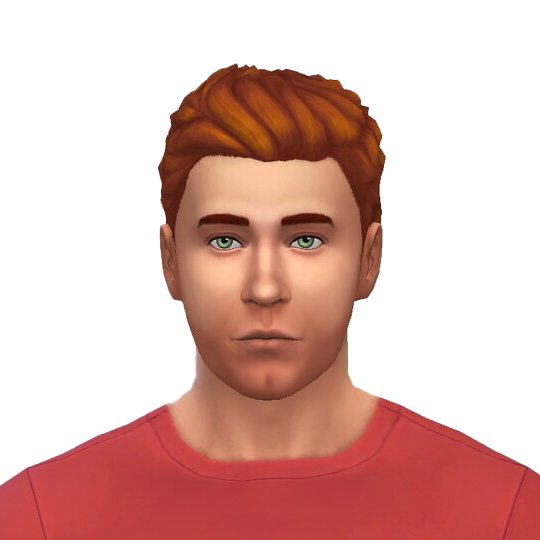
\includegraphics[height=5cm]{zdjęcia/1.png}
		\subcaption{\label{avatar_1}}
	\end{subfigure}
	\begin{subfigure}{0.35\textwidth}
		\centering
		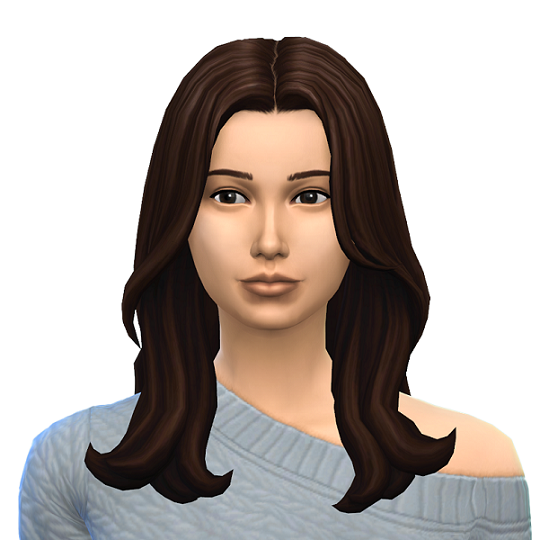
\includegraphics[height=5cm]{zdjęcia/2.png}
		\subcaption{\label{avatar_2}}
	\end{subfigure}
	\begin{subfigure}{0.35\textwidth}
		\centering
		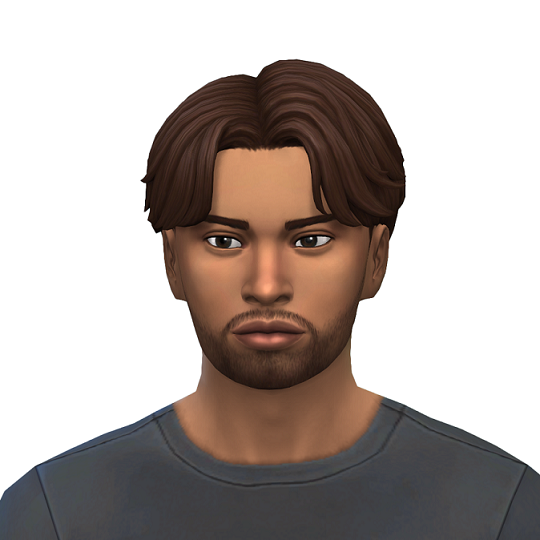
\includegraphics[height=5cm]{zdjęcia/3.png}
		\subcaption{\label{avatar_3}}
	\end{subfigure}
	\begin{subfigure}{0.35\textwidth}
		\centering
		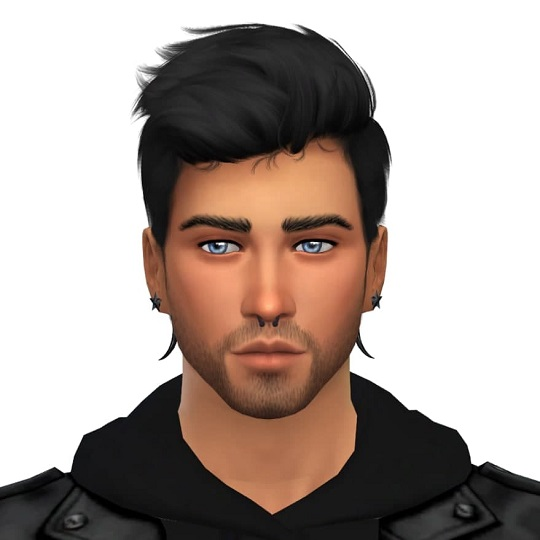
\includegraphics[height=5cm]{zdjęcia/4.png}
		\subcaption{\label{avatar_4}}
	\end{subfigure}
	
	\caption{\label{fig:avatars}Awatary użyte do przetestowania algorytmu}
\end{figure}

% %---------------------------------------------------------------------------

\section{Walidacja z użyciem aplikacji}
Pierwsza część wykonanych testów objęła wykorzystanie aplikacji webowej w celu zbadania efektywności działania algorytmu w przypadku animacji na podstawie obrazu przechwyconego z kamery. 

Na potrzeby przeprowadzonego badania stworzono ankietę składającą się z czterech sekcji, gdzie każda dotyczy modyfikacji innego awatara. Głównym zadaniem miała być ocena rezultatów odwzorowania czterech podstawowych emocji \cite{emotions}, na które składają się:

\begin{itemize}
    \item szczęście,
    \item smutek,
    \item strach/zaskoczenie,
    \item gniew/obrzydzenie.
\end{itemize}

Każda sekcja złożona jest z pięciu pytań:
\begin{itemize}
    \item cztery z nich dotyczą testowania zakładki \textit{Real-time animation}, gdzie awatar jest animowany na podstawie obrazu przechwyconego z kamery,
    \item jedno ma na celu porówananie efektów otrzymanych przez animację opartą na analizowaniu obrazu z kamery z modyfikacją na podstawie wczytanego zdjęcia (zakładka \textit{Select image}).
\end{itemize}

Treść czterech pierwszych pytań, pod którymi kryją się kolejne zadania, różni się między sobą tylko aktualnie testowaną emocją. Dla przykładu pierwsze pytanie ma postać:
\begin{center}
    Odwzorowanie pierwszej podstawowej emocji (szczęście).
\end{center}

W tej części zastosowano ocenianie za pomocą skali od 1 do 5, gdzie konkretnym wartościom odpowiadały następujące etykiety:
\begin{enumerate}
    \item Bardzo słaby
    \item Słaby
    \item Przeciętny
    \item Dobry
    \item Bardzo dobry

\end{enumerate}

Ostatnie, piąte pytanie dotyczy oceny rezultatu osiągniętego w zakładce \textit{Select image} dla danego awatara. Osoba ankietowana powinna wybrać jedno zdjęcie z udostępnionej bazy, odwzorowujące emocje, dla której animacja wypadła najgorzej. Następnie należało ocenić osiągnięty efekt, w stosunku do tego otrzymanego w zakładce \textit{Real-time animation}. Tym razem użyto skali od 1 do 7 gdzie 1 oznacza \textit{zdecydowanie gorszy} efekt, natomiast 7 \textit{zdecydowanie lepszy} wynik.

Przed przystąpieniem do testowania użytkownicy zostali zapoznani z krótką instrukcją, w której zwrócono uwagę na czynniki mogące mieć wpływ na działanie algorytmu:

\begin{enumerate}
    \item Ustaw twarz w pozycji frontowej, tak aby była ona dobrze widoczna w kamerze.
    \item Odsłoń włosy oraz zdejmij okulary.
    \item Staraj się nie wykonywać gwałtownych ruchów w momencie naciskania przycisku \textit{Animate}.
    \item W trakcie oceny rezultatów kieruj się głównie tym, czy emocja została poprawnie odwzorowana.
    \item Możesz wielokrotnie dokonywać animacji dla danej emocji i ocenić sumaryczne rezultaty.
\end{enumerate}

W ankiecie wzięło udział 11 osób w przedziale wiekowym od 19 do 60 lat. Większość z nich korzysta na co dzień z komputera, jednak tylko w podstawowych celach. W trakcie przeprowadzania ankiety nie wyniknęły żadne problemy. Aplikacja działała płynnie, przez co każdej ankietowanej osobie udało się ukończyć zadania bez przeszkód.

\begin{table}[h]
\centering
\begin{tabular}{|c|l|c|c|c|c|c|} 
\hline
\multirow{2}{*}{\textbf{awatar}} & \multicolumn{1}{c|}{\multirow{2}{*}{\textbf{emocja}}} & \multicolumn{5}{c|}{\textbf{ocena}}                                                                                                   \\ 
\cline{3-7}
                                 & \multicolumn{1}{c|}{}                                 & \textbf{1} & \textbf{2} & \textbf{3}                       & \textbf{4}                         & \textbf{5}                          \\ 
\hhline{|=======|}
\multirow{4}{*}{\ref{avatar_1}}        & szczęście                                             & ~ 0\%~~    & ~ 9\%~~    & ~ 0\%~                           & \textcolor[rgb]{0,0.588,0}{~ 45\%} & \textcolor[rgb]{0,0.588,0}{~ 45\%}  \\ 
\cline{2-7}
                                 & smutek                                                & 0\%        & 0\%        & 0\%                              & \textcolor[rgb]{0,0.588,0}{64\%}   & 36\%                                \\ 
\cline{2-7}
                                 & zaskoczenie/strach                                    & 0\%        & 0\%        & 18\%                             & \textcolor[rgb]{0,0.588,0}{45\%}   & 36\%                                \\ 
\cline{2-7}
                                 & gniew/obrzydzenie                                     & 0\%        & 9\%        & 18\%                             & \textcolor[rgb]{0,0.588,0}{36\%}   & \textcolor[rgb]{0,0.588,0}{36\%}    \\ 
\hhline{|=======|}
\multirow{4}{*}{\ref{avatar_2}}           & szczęście                                             & 0\%        & 9\%        & 9\%                              & \textcolor[rgb]{0,0.588,0}{45\%}   & 36\%                                \\ 
\cline{2-7}
                                 & smutek                                                & 0\%        & 27\%       & 9\%                              & \textcolor[rgb]{0,0.588,0}{45\%}   & 18\%                                \\ 
\cline{2-7}
                                 & zaskoczenie/strach                                    & 9\%        & 0\%        & 27\%                             & \textcolor[rgb]{0,0.588,0}{55\%}   & 9\%                                 \\ 
\cline{2-7}
                                 & gniew/obrzydzenie                                     & 9\%        & 18\%       & \textcolor[rgb]{0,0.588,0}{45\%} & 27\%                               & 0\%                                 \\ 
\hhline{|=======|}
\multirow{4}{*}{\ref{avatar_3}}          & szczęście                                             & 0\%        & 0\%        & 9\%                              & \textcolor[rgb]{0,0.588,0}{45\%}   & \textcolor[rgb]{0,0.588,0}{45\%}    \\ 
\cline{2-7}
                                 & smutek                                                & 0\%        & 0\%        & 27\%                             & \textcolor[rgb]{0,0.588,0}{55\%}   & 18\%                                \\ 
\cline{2-7}
                                 & zaskoczenie/strach                                    & 0\%        & 9\%        & 18\%                             & \textcolor[rgb]{0,0.588,0}{36\%}   & \textcolor[rgb]{0,0.588,0}{36\%}    \\ 
\cline{2-7}
                                 & gniew/obrzydzenie                                     & 0\%        & 18\%       & 18\%                             & \textcolor[rgb]{0,0.588,0}{36\%}   & 27\%                                \\ 
\hhline{|=======|}
\multirow{4}{*}{\ref{avatar_4}}         & szczęście                                             & 0\%        & 0\%        & 0\%                              & 18\%                               & \textcolor[rgb]{0,0.588,0}{82\%}    \\ 
\cline{2-7}
                                 & smutek                                                & 0\%        & 9\%        & 0\%                              & \textcolor[rgb]{0,0.588,0}{55\%}   & 36\%                                \\ 
\cline{2-7}
                                 & zaskoczenie/strach                                    & 0\%        & 9\%        & 9\%                              & \textcolor[rgb]{0,0.588,0}{55\%}   & 27\%                                \\ 
\cline{2-7}
                                 & gniew/obrzydzenie                                     & 0\%        & 9\%        & 9\%                              & \textcolor[rgb]{0,0.588,0}{64\%}   & 18\%                                \\
\hline
\end{tabular}
\caption{Wyniki walidacji przeprowadzonej z użyciem aplikacji webowej}
\label{tab:first_test}
\end{table}

Procentowe wyniki ankiety przedstawiono w powyższej tabeli~(Tab.~\ref{tab:first_test}). Zawarto w niej podsumowane odpowiedzi na pytania 1-4, czyli te dotyczące odwzorowania danej emocji. Dla każdego awatara i poszczególnych emocji dominujące wartości oznaczono kolorem zielonym. 

Analizując wyniki można dojść do następujących wniosków:
\begin{itemize}
    \item najlepsze oceny zanotowano dla awatara \ref{avatar_4}. Odwzorowanie każdej z emocji zostało ocenione jako \textit{dobre} lub \textit{bardzo dobre} średnio w 89\% przypadków,
    \item ocena \textit{bardzo słaby} pojawiła się dwukrotnie, wyłącznie dla awatara \ref{avatar_2},
    \item największa liczba ocen \textit{słaby} oraz \textit{bardzo słaby} wystąpiła dla awatara \ref{avatar_2} (średnio 18\% odpowiedzi).
\end{itemize}


Podsumowując odpowiedzi na ostatnie pytanie, dotyczące porównania efektów osiągniętych w zakładce \textit{Select image} oraz \textit{Real-time animation}, można zauważyć, że:
\begin{itemize}
    \item dla awatara \ref{avatar_1}, w 91\% przypadków, odpowiedzi skupiły się w przedziale od 4 do 7, co oznacza tendencję w kierunku \textit{zdecydowanie lepszego} efektu,
    \item oceny awatara \ref{avatar_2} kumulowały się między 1 a 4, przez co rozumie się osiągnięcie głównie gorszych rezultatów,
    \item dla awatara \ref{avatar_3} koncentracja odpowiedzi przypadła na przedział 4-7, aż w 45\% zdecydowano że efekt modyfikacji poprzez zakładkę \textit{Select image} jest \textit{zdecydowanie lepszy},
    \item efekty dla ostatniego awatara (\ref{avatar_4}) zostały ocenione bardzo różnorodnie, żadna z odpowiedzi nie wydaje się znacząco dominować.
\end{itemize}


% %---------------------------------------------------------------------------

\section{Walidacja na zbiorze danych}
Drugi etap testów dotyczył oceny rezultatów algorytmu osiągniętych z wykorzystaniem gotowego zbioru danych. Celem tej części była ocena wcześniej zmodyfikowanych awatarów. Powinna ona zapewnić przejrzyste, nieobarczone błędem wnioski. Wyniki walidacji przedstawionej we wcześniejszej sekcji są narażone na przekłamanie, ponieważ efekty zależały od mimiki poszczególnych osób biorących udział w badaniu.

Przygotowanie danych przebiegało w następujący sposób:
\begin{itemize}
    \item wykorzystano bazę zdjęć zawierającą podobizny mężczyzn oraz kobiet z różnymi wyrazami twarzy, odpowiadającymi określonym emocjom,
    \item dla każdej emocji, których podstawowy podział został podany w powyższym rozdziale, wybrano po jednym zdjęciu,
    \item na podstawie określonych obrazów dokonano modyfikacji każdego awatara. Finalnie otrzymano 16 przekształconych podobizn.
\end{itemize}


Ankieta utworzona na potrzeby badania składa się z  16 pytań, każde z nich posiada cztery możliwe odpowiedzi:

\begin{enumerate}
    \item szczęście,
    \item smutek,
    \item strach/zaskoczenie,
    \item gniew/obrzydzenie.
\end{enumerate}

Zadaniem osoby ankietowanej była próba dopasowania emocji, którą odzwierciedla zmodyfikowany wyraz twarzy awatara. W celu łatwiejszego uporządkowania wyników zastosowano punktację 0-1. 

W ankiecie wzięło udział 27 osób w różnym przedziale wiekowym. Poniżej przedstawiono wartości najważniejszych parametrów otrzymanych wyników:
\begin{itemize}
    \item maksymalna liczba zdobytych punktów - 16
    \item najniższy wynik - 9
    \item średni wynik - 12,44/16
    \item mediana - 12
\end{itemize}

\begin{table}[h]
\centering
\begin{tabular}{|c|c|c|c|c|} 
\hline & \multicolumn{4}{c|}{\textbf{awatar}} \\ 
\hline
\textbf{emocja} & \textbf{\ref{avatar_1}} & \textbf{\ref{avatar_2}} & \textbf{\ref{avatar_3}} & \textbf{\ref{avatar_4}} \\ 
\hline
szczęście & 74\% & 70\% & 85\% & \textcolor[rgb]{0,0.502,0}{\textbf{100\%}} \\ 
\hline
smutek & 78\% & \textcolor[rgb]{0,0.502,0}{~\textbf{93\%}} & 85\% & 85\% \\ 
\hline
zaskoczenie/strach & \textcolor[rgb]{0,0.502,0}{~\textbf{93\% }} & 74\% & 63\% & 63\% \\ 
\hline
gniew/obrzydzenie & 78\% & 41\% & \textcolor[rgb]{0,0.502,0}{~\textbf{96\%}} & 67\% \\ 
\hline
\bottomrule
\begin{tabular}[c]{@{}c@{}}sumaryczna poprawność\end{tabular} & 81\% & {\cellcolor{red}}\textcolor{white}{69\%}  & {\cellcolor[rgb]{0,0.502,0}}\textcolor{white}{82\%} & 79\% \\
\hline
\end{tabular}
\caption{Ocena rezultatów osiągniętych z użyciem gotowego zbioru danych}
\label{tab:second_test}
\end{table}

Wyniki procentowe otrzymane po przeprowadzeniu badania zawarto w tabeli \ref{tab:second_test}. Po szczegółowej analizie, można zauważyć, że:
\begin{itemize}
    \item najwyżej oceniono awatar \ref{avatar_3} (82\% poprawnych odpowiedzi), a najgorzej \ref{avatar_2} (poprawność na poziomie 69\%),
    \item w odwzorowaniu szczęścia najwyższy wynik, bo aż 100\% zanotowano dla awatara \ref{avatar_4},
    \item smutny wyraz twarzy najtrafniej przyporządkowywano dla awatara \ref{avatar_2} (93\%),
    \item w przypadku emocji zaskoczenia/strachu najwyższą poprawność dopasowania otrzymano dla awatara \ref{avatar_1} (93\%),
    \item najlepszy rezultat dla gniewu/obrzydzenia osiągnięto na awatarze \ref{avatar_3} (96\%).
\end{itemize}

Obrazy, których odzwierciedlane emocje przyporządkowano z najlepszą skutecznością (kolejno 100\% oraz 96\%) przedstawiono na Rys. \ref{fig:best_results}. Według ankietowanych obraz \ref{av-4_happiness_2} bardzo dobrze oddaje szczęście, mimo pewnego defektu w postaci braku uzębienia. Natomiast Rys.~\ref{av-3_anger_2} poprawnie ukazuje gniew/obrzydzenie poprzez odpowiednie ułożenie ust oraz oczu. 

\begin{figure}[h]
	\centering
	\begin{subfigure}{0.35\textwidth}
		\centering
		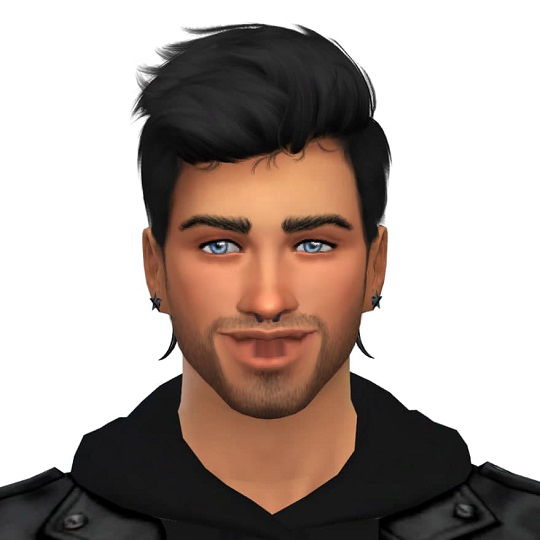
\includegraphics[height=5.5cm]{zdjęcia/av-4_happiness_2.png}
		\subcaption{\label{av-4_happiness_2}}
	\end{subfigure}
	\begin{subfigure}{0.35\textwidth}
		\centering
		
\includegraphics[height=5.5cm]{zdjęcia/av-3_anger_2.png}
		\subcaption{\label{av-3_anger_2}}
	\end{subfigure}

	
	\caption{\label{fig:best_results}Najtrafniej odgadnięte odwzorowania}
\end{figure}

% %---------------------------------------------------------------------------

\section{Wnioski}
Przeprowadzone testy pomogły sprawdzić poprawność działania algorytmu zaimplementowanego w niniejszej pracy dyplomowej. Według użytkowników algorytm zapewnia dobre efekty, a stworzona aplikacja jest intuicyjna w użyciu. Wiele osób stwierdziło, iż udział w badaniu był przyjemny i przysporzył sporo rozrywki.

Analiza przeprowadzona w powyższym rozdziale pozwoliła na wykrycie wad oraz zdefiniowanie potencjalnych kierunków rozwoju programu. Kilku użytkowników zwróciło uwagę na brak uzębienia animowanych awatarów, który rozpraszał w trakcie testowania algorytmu. Pojedyncze osoby wspomniały także o braku uwzględniania ułożenia brwi. Niewykluczone, że poprawa tego elementu zdecydowanie udoskonaliłaby odwzorowanie emocji, które można osiągnąć z użyciem owego oprogramowania.

Głównym celem ewaluacji było zbadanie jakości działania programu ze względu na dobór awatara. Okazało się, że efektywność narzędzia w dużym stopniu zależy od obrazu, na którym następuje animacja. W pierwszej części testów najwyżej oceniono obraz \ref{avatar_4}, natomiast w drugiej \ref{avatar_3}. Najniższe oceny, w obu przypadkach, pojawiły się dla awatara \ref{avatar_2}. Podczas jego modyfikacji można było zauważyć sporo artefaktów psujących efekt animacji. Jak widać, mimo wykorzystania identycznych obrazów, dla różnych awatarów otrzymano odmienne wyniki. W przypadku kobiety znajdującej się na obrazie \ref{avatar_2} włosy nachodzące na twarz mogły negatywnie wpłynąć na rezultaty.

Istotną kwestią była także część, w której porównywano działanie oprogramowania na gotowych obrazach z animacją na podstawie obrazu przechwyconego z kamery. Dla awatarów ocenionych najwyżej osiągnięte efekty były zbliżone. Dla awatara ocenionego najgorzej efektywność animacji na podstawie gotowych obrazów dawała lepsze wyniki. Można z tego wnioskować, iż poprawnie wykonana animacja z użyciem kamery nie wpływa negatywnie na wizualicję, a w przypadku animacji niekorzystnego awatara może poprawić jej efekt. Nie należy jednak zapominać, że efekty są mocno zależne od mimiki danej osoby - dla każdej z nich inny awatar może sprawdzić się lepiej. 

Uważam, iż przeprowadzone testy przebiegły pomyślnie. Stworzona aplikacja okazała się dobrym narzędziem walidacji. Ewaluacja na gotowym zbiorze danych pomogła zweryfikować otrzymane wnioski oraz zwrócić uwagę na inne ścieżki rozwoju.



